\documentclass[a4paper, 10pt, garamond, oneside]{book}
\usepackage{cours-preambule}

\toggletrue{student}
\HideSolutionstrue

\makeatletter
\renewcommand{\@chapapp}{MPSI3 -- 29 septembre 2023 -- Devoir surveillé}
\makeatother

\graphicspath{{./figures/}{./figures/E1}{./figures/E2}{./figures/P1}{./figures/P2}}

\setlist[enumerate]{resume}
\setlist[enumerate,1]{leftmargin=10pt, label=\sqenumi}
\setlist[enumerate,2]{leftmargin=20pt, label=\Alph*)}

\newcommand{\figsvg}[1]{
  \begin{center}
    \subimport{figures/}{#1}
  \end{center}
}
\newcommand{\figsvgCap}[2]{
  \begin{center}
    \subimport{figures/}{#1}
    \captionof{figure}{#2}
  \end{center}
}

\begin{document}
\setcounter{chapter}{0}
\chapter{Électrocinétique\ifprof{\!\!-- corrigé}}
\label{ch:ds02}

\ifstudent{
\begin{center}
	\Large\bfseries
	\xul{Tout moyen de communication est interdit}
	\smallbreak
	\xul{Les téléphones portables doivent être éteints et rangés dans les sacs}
	\smallbreak
	\xul{Les calculatrices sont \textit{interdites}}
\end{center}
\begin{prgm}
	\vspace{6pt}
	\begin{tcb}*[cnt, bld, fontupper=\large](ror){}
		Électrocinétique, résistances et sources, circuits RC et RL
	\end{tcb}
	\vspace{-8pt}
\end{prgm}
Le devoir est composé des parties \textit{indépendantes} suivantes~:
{\Large
\begin{itemize}[label=$\diamond$]
	\bitem{Exercice 1}~: Modélisation d'un dipôle linéaire
	\bitem{Exercice 2}~: Point de fonctionnement d'une diode
	\bitem{Problème 1}~: Balise lumineuse
	\bitem{Problème 2}~: Régimes transitoires successifs d'un circuit RL
\end{itemize}
}

Les différentes questions peuvent être traitées dans l'ordre désiré.
\textbf{Cependant}, le numéro complet de la question doit être indiqué, et
\textbf{vous indiquerez si vous traitez la question d'un exercice sur une page
	complètement déconnectée}, sous peine de n'être ni vue ni corrigée.
\bigbreak
Une attention particulière sera portée à la \textbf{qualité de rédaction}. Les
hypothèses doivent être clairement énoncées, les propositions reliées entre
elles par des connecteurs logiques, les lois et théorèmes énoncés, sans pour
autant devenir une composition de français.
\bigbreak
De plus, la \textbf{présentation} de la copie sera prise en compte. Outre la
numérotation des questions, l'écriture, l'orthographe, les encadrements, la
marge, le cadre laissé pour la note et le commentaire font partie des points à
travailler. Il est notamment attendu que \textbf{les expressions littérales
	soient encadrées}, que \textbf{les calculs n'apparaissent pas} mais que le
détail des grandeurs avec leurs unités soit indiqué, et \textbf{les applications
	numériques soulignées}.
\bigbreak
Ainsi, l'étudiant-e s'expose aux malus suivants concernant la forme et le fond~:
\begin{tcb}*(prop)"bomb"{Malus}
	\begin{minipage}{0.50\linewidth}
		\begin{itemize}
			\item A~: application numérique mal faite~;
			\item N~: numéro de copie manquant~;
			\item P~: prénom manquant~;
			\item E~: manque d'encadrement des réponses~;
			\item M~: marge non laissée ou trop grande~;
			\item V~: confusion ou oubli de vecteurs~;
		\end{itemize}
	\end{minipage}
	\begin{minipage}{0.50\linewidth}
		\begin{itemize}
			\item Q~: question mal ou non indiquée~;
			\item C~: copie grand carreaux~;
			\item U~: mauvaise unité (flagrante)~;
			\item H~: homogénéité non respectée~;
			\item S~: chiffres significatifs non cohérents~;
			\item $\f$~: loi physique fondamentale brisée.
		\end{itemize}
	\end{minipage}
\end{tcb}

\begin{tcb}(impo){Exemple application numérique}
	\vspace*{-10pt}
	\begin{minipage}{0.45\linewidth}
		\begin{gather*}
			\boxed{n = \frac{PV}{RT}}
			\qav
			\left\{
			\begin{array}{rcl}
				p & = & \SI{1.0e5}{Pa}                \\
				V & = & \SI{1.0e-3}{m^3}              \\
				R & = & \SI{8.314}{J.mol^{-1}.K^{-1}} \\
				T & = & \SI{300}{K}
			\end{array}
			\right.\\
			\mathrm{A.N.~:}\quad
			\xul{n = \SI{5.6e-4}{mol}}
		\end{gather*}
	\end{minipage}
	\hfill
	\cancel{\bcancel{
			\begin{minipage}{0.45\linewidth}
				\begin{gather*}
					n = \frac{PV}{RT} = \frac{\num{e5}\cdot\num{1}}{8.32\cdot300}
					= 0.56
				\end{gather*}
			\end{minipage}
		}}
\end{tcb}
\newpage
}

\setcounter{section}{0}
\exercice[30]{Modélisation d'un dipôle linéaire}
\restartlist{enumerate}

\ifstudent{
	Dans ce problème, on étudie le dipôle $A B$ suivant dans lequel
	le dipôle $D$ peut être un fil, un interrupteur
	ouvert ou une résistance.

	\begin{figure}[htbp]
		\centering
		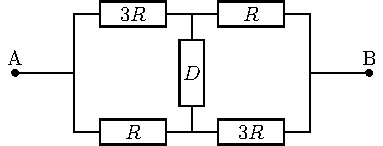
\includegraphics[scale=1]{diplin_1}
		\label{fig:diplin1}
	\end{figure}
}
\switch{
	\begin{enumerate}
		\item Exprimer la résistance $R_\infty$ du dipôle $A B$
		      si $D$ est un interrupteur ouvert.
		      Faire l'application numérique.
		\item Exprimer la résistance $R_0$ du dipôle $A B$
		      si $D$ est un fil.
		      Faire l'application numérique.
	\end{enumerate}
}{
	\begin{enumerate}
		\item
		      \noindent
		      \begin{minipage}{0.6\linewidth}
			      Si $D$ est un interrupteur ouvert, alors le circuit est composé de
			      deux branches de résistance $4R$ en parallèle, donc
			      $\boxed{R_\infty=2R=\SI{200}{\ohm}}$.
		      \end{minipage}
		      \begin{minipage}{0.4\linewidth}
			      \begin{center}
				      FIGURE
			      \end{center}
		      \end{minipage}
		\item
		      \noindent
		      \begin{minipage}{0.6\linewidth}
			      Si $D$ est un fil, le circuit est l'association en série de deux
			      résistances $R_{eq}$ identiques correspondant à l'association en
			      parallèle de la résistance $3R$ et de la résistance $R$.
			      Donc $R_{eq}=3R/4$ et $\boxed{R_0=3R/2=\SI{150}{\ohm}}$.
		      \end{minipage}
		      \begin{minipage}{0.4\linewidth}
			      \begin{center}
				      \figRaw{fig1corr2}
			      \end{center}
		      \end{minipage}
	\end{enumerate}
}
\subsection{Sur une source de tension}
\switch{
	Dans cette partie, le dipôle $A B$ est branché 	sur une source de tension de
	force électromotrice constante $E$.
	Toutes les notations utilisées dans cette partie sont définies sur le schéma
	suivant.
	\begin{center}
		FIGURE2
	\end{center}
	\begin{center}
		\bfseries
		Dans cette partie, les expressions littérales ne pourront faire intervenir
		que $E$ et $R$.
	\end{center}
	\begin{enumerate}[resume]
		\item Exprimer la tension $u$ si 	$D$ est un interrupteur ouvert.
		      Faire l'application numérique.
	\end{enumerate}
	Pour les deux questions suivantes, D est un \textbf{interrupteur fermé}.
	\begin{enumerate}[resume]
		\item
		      Exprimer la tension $v$ dans ce cas. Faire l'application numérique.
		\item
		      Exprimer l'intensité $i$  dans ce cas. Faire l'application numérique.
	\end{enumerate}

}{
	\begin{enumerate}[resume]
		\item
		      \noindent
		      \begin{minipage}{0.4\linewidth}
			      Par additivité des tensions, $u=v'-v$. On reconnait deux ponts
			      diviseurs de tension :
			      \eq{
				      v'=\frac{3E}{4}\quad;\quad v=\frac{E}{4}
			      }
			      \eq{
				      \boxed{u=\frac{E}{2}=\SI{3}{\volt}}
			      }
		      \end{minipage}
		      \begin{minipage}{0.6\linewidth}
			      \begin{center}
				      \figRaw{fig2corr}
			      \end{center}
		      \end{minipage}
		\item
		      La tension $v$ correspond à la tension aux bornes de la résistance
		      équivalente $R_{eq}$ (voir figure de la question 2).

		      On applique la formule du pont diviseur de tension sur l'association
		      en série des deux résistances $R_{eq}$~:
		      $\boxed{v=E/2=\SI{3}{\volt}}$.
		\item
		      \noindent
		      \begin{minipage}{0.4\linewidth}
			      Par l'application de la loi des nœuds et de la loi d'Ohm :
			      \eq{
				      i=i_2-i_1=\frac{v}{R}-\frac{v}{3R}
			      }

			      \eq{
				      \boxed{i=\frac{E}{3R}=\SI{20}{\milli\ampere}}
			      }
		      \end{minipage}
		      \begin{minipage}{0.6\linewidth}
			      \begin{center}
				      \figRaw{fig2corr2}
			      \end{center}
		      \end{minipage}
	\end{enumerate}
}
\subsection{Sur une source de courant}
\switch{
	Dans cette partie, le dipôle $A B$ est branché
	sur une source de courant, dont le courant électromoteur $I_0$ est
	constant.
	Toutes les notations utilisées dans cette partie sont
	définies sur le schéma suivant.

	\begin{center}
		FIGURE 3
	\end{center}

	\begin{center}
		\bfseries
		Dans cette partie, les expressions littérales
		ne pourront faire intervenir que $I_0$ et $R$.
	\end{center}
	\begin{enumerate}[resume]
		\item
		      Exprimer la tension $u$ si 	$D$ est un interrupteur ouvert.
		      Faire l'application numérique.
	\end{enumerate}
	Pour les deux questions suivantes, D est un \textbf{interrupteur fermé}.
	\begin{enumerate}[resume]
		\item
		      Exprimer l'intensité $i''$. Faire l'application numérique.
		\item
		      Exprimer l'intensité $i$ dans ce cas. Faire l'application numérique.
	\end{enumerate}
}{
	\begin{enumerate}[resume]
		\item
		      \noindent
		      \begin{minipage}{0.4\linewidth}
			      Si $D$ est un interrupteur ouvert, alors le courant est le même
			      dans les deux branches qui ont la même résistance équivalente,
			      donc $i''=I_0/2$.
			      Par l'additivité des tensions, $u=u'-u''$.
			      En appliquant la loi d'Ohm, on obtient
			      $\boxed{u=RI_0=\SI{4}{\volt}}$.
		      \end{minipage}
		      \begin{minipage}{0.6\linewidth}
			      \begin{center}
				      \figRaw{fig3corr2}
			      \end{center}
		      \end{minipage}
		\item
		      On applique la formule du pont diviseur de courant
		      $\boxed{i''=3I_0/4=\SI{30}{\milli\ampere}}$.
		\item
		      \noindent
		      \begin{minipage}{0.4\linewidth}
			      D'après la formule du pont diviseur de courant $i_R=-I_0/4$. Par
			      la loi des nœuds $\boxed{\cfrac{I_0}{2}=\SI{20}{\milli\ampere}}$.
		      \end{minipage}
		      \begin{minipage}{0.6\linewidth}
			      \begin{center}
				      \figRaw{fig3corr}
			      \end{center}
		      \end{minipage}
	\end{enumerate}
}
\subsection{Application}
\switch{
	On admet qu'il existe quatre constantes $a$, $b$, $c$ et $d$ telles que
	\begin{align*}
		u' & =a i + b u \\
		i' & = c i + du
	\end{align*}
	quels que soient les dipôles $D$ et $D'$ dans le circuit suivant.
	\begin{center}
		FIGURE 4
	\end{center}
	\begin{enumerate}[resume]
		\item
		      Exprimer les constantes $a$, $b$, $c$ et $d$.
	\end{enumerate}
	Pour les deux questions suivantes, D est une résistance $\rho$
	\begin{enumerate}[resume]
		\item Exprimer la résistance équivalente $R_\rho$ du dipôle $A B$ en
		      fonction des résistances $R$ et $\rho$.
		\item
		      Que devient l'expression précédente dans la limite $\rho \ra \infty$~?
		      Commenter.
		\item
		      Que devient l'expression précédente dans la limite $\rho \ra 0$~?
		      Commenter.
	\end{enumerate}

}{
	\begin{enumerate}[resume]
		\item
		      Dans le cas où $D'$ est un générateur de tension de f.e.m. $u'=E$ :
		      \begin{itemize}
			      \item Si $D$ est un interrupteur ouvert, $i=0$ et $u=E/2$~:
			            $E=bE/2$, donc $\boxed{b=2}$
			      \item Si $D$ est un fil, $u=0$ et $i=E/(3R)$~: $E=aE/(3R)$, donc
			            $\boxed{a=3R}$
		      \end{itemize}

		      Dans le cas où $D'$ est un générateur de courant de c.e.m. $i'=I_0$ :
		      \begin{itemize}
			      \item Si $D$ est un fil, $u=0$ et $i=I_0/2$ : $I_0=cI_0/2$,
			            donc $\boxed{c=2}$
			      \item Si $D$ est un interrupteur ouvert, $i=0$ et $u=RI_0$~:
			            $I_0=dRI_0$, donc $\boxed{d=1/R}$
		      \end{itemize}
		\item $\lim_{\rho\rightarrow \infty }R_\rho=2R=R_\infty$, il y a cohérence
		      avec la réponse à la question 1.
		\item $\lim_{\rho\rightarrow 0}R_\rho=3R/2=R_0$, il y a cohérence avec la
		      réponse à la question 2.
	\end{enumerate}
}

\newpage

\exercice[30]{Point de fonctionnement d'une diode}
\restartlist{enumerate}

\switch{
	On considère une diode en silicium dont la caractéristique courant/tension est représentée sur la figure~\ref{fig:carac_diode}. La diode est dite bloquée quand la tension à ses bornes $u_D$ est inférieure à sa tension seuil $u_s$. La diode est dite passante dans le cas contraire.

	On prendra $u_s=\SI{0,60}{\volt}$. On donne les coordonnées du point $C$ : $i_C=\SI{500}{\milli\ampere}$ et $u_C=\SI{0,70}{\volt}$.

	\noindent
	\begin{minipage}[t]{.5\linewidth}
		\begin{center}
			\subimport{figures/E2/}{diode_carac.pdf_tex}
			\captionof{figure}{Caractéristique d'une diode silicium.}
			\label{fig:carac_diode}
		\end{center}
	\end{minipage}
	\begin{minipage}[t]{.5\linewidth}
		\begin{center}
			\subimport{figures/E2/}{diode_thevenin.pdf_tex}
			\captionof{figure}{Modèle de \textsc{Thévenin}}
			\label{fig:thevenin}
		\end{center}
	\end{minipage}
	\begin{enumerate}
		\item Dans le cas où la diode est bloquée, par quel dipôle peut-on la
		      modéliser~?
		\item Dans le cas où la diode est passante, le courant vérifie
		      $i_D=a\cdot u_D+b$. Exprimer $a$ et $b$ en fonction de $u_s$, $i_C$
		      et $u_C$. Calculer $a$ et $b$.
	\end{enumerate}

	On veut montrer que la diode peut être modélisée par un générateur de
	Thévenin de f.e.m. $e$ et de résistance $r$ (figure~\ref{fig:thevenin})
	lorsqu'elle est passante.
	\begin{enumerate}[resume]
		\item Exprimer $i$ en fonction de $u$, $e$ et $r$.
		\item En déduire les expressions de $e$ et $r$ en fonction de $a$ et $b$ pour que la diode soit équivalente au générateur de Thévenin lorsqu'elle est passante. Calculer $e$ et $r$.
	\end{enumerate}
	On considère le circuit de la figure~\ref{fig:circuit_diode1} constitué de la diode précédente, d'un générateur de tension idéal de f.e.m. $e_1$ et de deux résistances identiques $R$.
	\smallbreak
	\noindent
	\begin{minipage}[t]{.5\linewidth}
		\begin{center}
			\subimport{figures/E2/}{diode_1.pdf_tex}
			\captionof{figure}{Circuit électrique étudié.}
			\label{fig:circuit_diode1}
		\end{center}
	\end{minipage}
	\begin{minipage}[t]{.5\linewidth}
		\begin{center}
			\subimport{figures/E2/}{diode_1.pdf_tex}
			\captionof{figure}{Étude du dipôle générateur.}
			\label{fig:circuit_diode2}
		\end{center}
	\end{minipage}
	\begin{enumerate}[resume]
		\item On suppose que la diode est bloquée. Refaire le circuit électrique. En déduire l'inégalité vérifiée par $e_1$ pour que cette hypothèse soit vérifiée.
		\item On suppose que la diode est passante. Refaire le circuit. Exprimer $u_D$ en fonction de $e_1$, $e$, $R$ et $r$. Calculer $u_D$ avec $e_1=\SI{10}{\volt}$ et $R=\SI{4.0}{\ohm}$. En déduire la valeur de $i_D$.
	\end{enumerate}

	On souhaite retrouver ce résultat graphiquement en utilisant le point de fonctionnement.
	\begin{enumerate}[resume]
		\item Exprimer $i'$ en fonction de $u'$ pour le circuit représenté sur la figure~\ref{fig:circuit_diode2}.
		\item En déduire graphiquement les coordonnées du point de fonctionnement en utilisant le document en annexe. Conclure.
	\end{enumerate}
}
{
	\begin{enumerate}
		\item Une diode bloquée est modélisable par un interrupteur ouvert ($i=0$).
		\item Le coefficient directeur est donné par le taux d'accroissement
		      $\boxed{a=\cfrac{i_C}{u_C-u_s}=\SI{5.0}{\siemens}}$.

		      Pour déterminer l'ordonnée à l'origine, on utilise le point
		      d'abscisse $u_s$ et d'ordonnée nulle :
		      \[
			      0=au_s+b\qsoit
			      \boxed{b=-au_s=\cfrac{-i_Cu_s}{u_C-u_s}=\SI{-3.0}{\ampere}}
		      \]
		\item D'après l'additivité des tensions et la loi d'Ohm, $u=ri-e$, soit
		      $\boxed{i=e/r+u/r}$.
		\item Deux dipôles sont équivalents s'ils ont la même caractéristique. On
		      en déduit $i=i_D$ $\forall u=u_D$, soit $e/r=b$ et $1/r=a$. Donc
		      $\boxed{e=b/a=-u_s=\SI{-0,60}{\volt}}$ et $\boxed{r=1/a=\SI{0,20}{\ohm}}$.
		\item En remplaçant la diode par un interrupteur, on reconnait un pont
		      diviseur de tension : $u_D=\cfrac{e_1}{2}$. La diode est bloquée si
		      $u_D<u_s$, donc il faut que $\boxed{e_1<2us}$.
		      \begin{center}
			      \subimport{figures/E2/}{diode_corr3.pdf_tex}
		      \end{center}
		\item On refait le circuit en faisant attention à l'orientation de la
		      tension $e$.
		      \begin{center}
			      \subimport{figures/E2/}{diode_corr.pdf_tex}
		      \end{center}

		      La loi des nœuds et les lois d'Ohm sont appliquées sur le schéma.
		      On définit $u_D$ comme étant la tension aux bornes des trois
		      branches en parallèle :

		      \begin{align}
			      u_D & =e_1-Ri_1\label{eq_uD1}   \\
			      u_D & =R(i_1-i_D)\label{eq_uD2} \\
			      u_D & =ri_D-e\label{eq_uD3}
		      \end{align}


		      \[
			      (\ref{eq_uD1})+(\ref{eq_uD2}) : 2u_D=e_1-Ri_D
			      \qsoit  i_D=\cfrac{e_1-2u_D}{R}
		      \]

		      \[
			      (\ref{eq_uD3}) : u_D=\cfrac{r}{R}(e_1-2u_D)-e
			      \qsoit \boxed{u_D=\frac{re_1-Re}{2r+R}=\SI{1.0}{\volt}}
		      \]

		      On remarque que $u_D>u_s$, donc la diode est bien passante.

		      Pour trouver $i_D$ on utilise la caractéristique de la diode~:
		      \[
			      \boxed{i_D=au_D+b=5\times 0,67-3=\SI{2.0}{\ampere}}
		      \]

		\item Loi des nœuds : $i'=i_1-i_2$

		      Loi des mailles et loi d'Ohm : $u'=e_1-Ri_1=Ri_2$

		      On en déduit : $i_1=\cfrac{e_1-u'}{R}$ et $i_2=u'/R$.

		      On remplace dans la loi des nœuds~:
		      $\boxed{i'=\cfrac{e_1}{R}-\cfrac{2}{R}u'}$

		      \begin{center}
			      \subimport{figures/E2/}{diode_corr2.pdf_tex}
		      \end{center}
		\item On lit les coordonnées du point d'intersection
		      $I(\SI{1.0}{\volt},\SI{2.0}{\ampere})$. Cela correspond aux valeurs
		      déterminées précédemment.
		      \begin{figure}[htbp]
			      \centering
			      \includegraphics[scale=1]{annexecorr}
		      \end{figure}
	\end{enumerate}
}

\newpage

\setcounter{section}{0}
\prblm[30]{Balise lumineuse}
\restartlist{enumerate}
\switch{
	\noindent
	\begin{minipage}[t]{.5\linewidth}
		~
		\begin{center}
			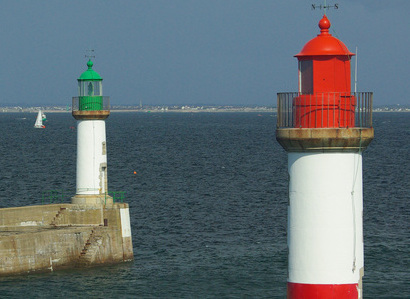
\includegraphics[width=.65\linewidth]{balise_photo}
		\end{center}
	\end{minipage}
	\hfill
	\begin{minipage}[t]{.5\linewidth}
		~
		\begin{center}
			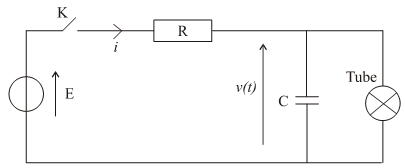
\includegraphics[width=.9\linewidth]{balise_schema_bis}
		\end{center}
	\end{minipage}
	\smallbreak
	La passe des ports est signalée la nuit par une balise lumineuse dont le
	schéma électrique est donné ci-dessus.
	La source de lumière est constituée d'un tube à décharge. La décharge
	électrique qui se produit entre les électrodes du tube est caractérisée par
	une tension d'allumage $U_{a}$ et
	une tension d'extinction $U_{ex}$.
	\bigbreak
	Le tube s'allume lorsque la tension à ses bornes prend une valeur qui devient
	supérieure à $U_{a}$, il se comporte alors comme un résistor de résistance
	$r \ll R$.
	\bigbreak
	Il s'éteint lorsque la tension à ses bornes prend une valeur qui devient
	inférieure à $U_{ex}$, il se comporte alors comme un résistor de résistance
	supposée infinie.
	\bigbreak
	Il s'allume à nouveau lorsque la tension à ses bornes redevient supérieure à
	$U_{a}$.
	\bigbreak
	On suppose que $E > U_{a}  > U_{ex}$ et on pose $\tau = RC$ ainsi que
	$\tau' = rC$.
	\smallbreak
	À l'instant initial $t = 0$, le condensateur n'est pas chargé et on ferme
	l'interrupteur $K$.
	\bigbreak
	Ainsi, lors de la charge du condensateur de constante de temps $\tau$, le tube
	est éteint (sa résistance est infinie), et lors de la décharge très rapide de
	constante de temps $\tau'$ à travers le tube (sa résistance est alors $r$), le
	tube est allumé.
	\begin{enumerate}
		\item
		      Déterminer le comportement du tube à l'instant initial.
		      En déduire le schéma équivalent du circuit et l'équation différentielle vérifiée par $v(t)$, puis la résoudre.
		\item
		      Déterminer l'expression de l'instant $t_{a}$  où s'amorce la décharge (allumage du tube).
		\item
		      On se place maintenant dans le régime où la lampe est allumée. Le circuit électrique est alors modifié et il convient de déterminer la nouvelle équation différentielle. Montrer que l'équation différentielle à laquelle satisfait $v(t)$ à partir de cet instant s'écrit avant simplification :
		      \[
			      E = RC \dv{v}{t} + \left(\frac{R}{r}+1\right) v
		      \]

		      \noindent
		      On utilisera la condition $r \ll R$ pour simplifier l'expression. Et on supposera que $v(t) \gg (r/R)E$ durant cette phase. Montrer que l'expression précédente devient alors
		      \[
			      0 = rC \dv{v}{t} + v
		      \]
		      \noindent
		      En déduire alors l'expression de $v(t)$.
		\item
		      Déterminer l'expression de l'instant $t_{ex}$ où se produit l'extinction du tube.
		\item
		      En déduire l'expression de la durée $T_1$ de l'éclair produit dans le tube.
		\item
		      Déterminer l'expression du temps $T_2$ qui s'écoule entre l'extinction et l'allumage suivant en fonction de $\tau$, $E$, $U_{ex}$  et $U_{a}$.
		\item
		      En déduire l'expression de la période $T$ des éclairs produits par ce dispositif.
		\item
		      Numériquement, on obtient
		      \[
			      \boxed{	T_1 = \SI{2,5e-7}{\second} \quad , \quad T_2 = \SI{1,0}{\second} \qet T = \SI{1,0}{\second}}
		      \]
		      Que peut-on en conclure~?
	\end{enumerate}
}{
	\begin{enumerate}
		\item
		      La tension aux bornes d'un condensateur est une fonction continue du temps donc $v(t=0^+)=v(t=0^-)=0<U_{a}$. Le tube est par conséquent éteint et la lampe est donc assimilable à un interrupteur ouvert. Le circuit devient donc :

		      \begin{figure}[htbp]
			      \centering
			      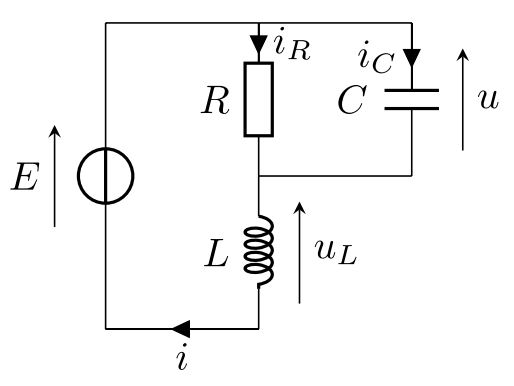
\includegraphics[width=.4\linewidth]{corrige1}
		      \end{figure}

		      Loi des mailles : $E = u_{R}(t) + v(t)$ \\
		      Loi d'Ohm : $u_{R}(t) = Ri(t) \quad \Rightarrow \quad E = Ri(t) + v(t)$ \\
		      Loi intensité/tension pour C : $i(t)=C \dv{v}{t} \quad \Rightarrow \quad E = RC \dv{v}{t} + v(t)$

		      La solution générale est la somme de la solution homogène et d'une solution
		      particulière constante :

		      \[
			      v(t) = A \exr^{-t/\tau} +E \qet \tau = RC
		      \]
		      $A$ se détermine avec les conditions initiales $v(t=0) = 0$. Ainsi,
		      \[
			      v(0) = A +E = 0 \qdc  A= -E
		      \]
		      Finalement~:
		      \[
			      \boxed{v(t) = E\left(1-\exr^{-t/\tau}\right)}
		      \]
		\item
		      La décharge s'amorce à l'instant $t_{a}$ tel que $v(t_{a}) =
			      U_{a}$. Soit

		      \[
			      E\left(1-\exr^{-t_{a}/\tau}\right) = U_{a}
		      \]

		      Après calcul, il vient~:
		      \[
			      \boxed{t_{a} = \tau \ln()\frac{E}{E-U_{a}})}
		      \]
		\item
		      La lampe est maintenant assimilable à une résistance $r$. On obtient
		      alors le nouveau schéma équivalent :

		      \begin{figure}[htbp]
			      \centering
			      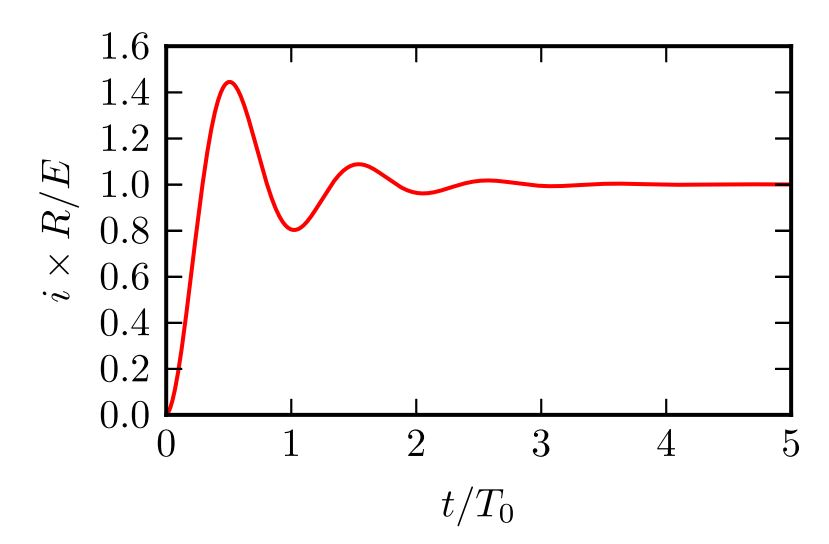
\includegraphics[width=.5\linewidth]{corrige2}
		      \end{figure}

		      L'équation différentielle s'obtient alors :

		      Loi des mailles : $E = u_{R}+v$

		      Loi d'Ohm: $E=Ri+v$

		      Loi des nœuds: $E = R(i_1+i_2)+v$

		      Loi intensité/tension aux bornes de r//C :
		      $E = R\pa{C\dv{v}{t}+ \frac{v}{r}}+v$

		      Il vient finalement,
		      \[
			      \frac{r}{R}E = rC\dv{v}{t}+ \left(1+\frac{r}{R}\right)v
			      \quad \Longleftrightarrow \quad
			      E = RC \dv{v}{t} + \left(\frac{R}{r}+1\right) v
		      \]

		      En négligeant les termes en $r/R$ : $0 = rC \dv{v}{t}+ v$

		      La solution s'écrit :
		      \[
			      v(t) = A \exr^{-t/\tau'} \qet \tau' = rC
		      \]
		      En exploitant la nouvelle condition initiale
		      $v(t=t_{a}) = U_{a}$, il vient
		      \[
			      A\exr^{-t_{a}/\tau'} =
			      U_{a} \qsoit  A =
			      U_{a}\exr^{t_{a}/\tau'}
		      \]
		      Ainsi,
		      \[
			      \boxed{v(t) = U_{a} \exr^{-(t-t_{a})/\tau'}}
		      \]
		\item
		      La décharge se termine à l'instant $t_{ex}$ tel que
		      $v(t_{ex}) = U_{ex}$. Soit

		      \[
			      U_{a} \exr^{-(t_{ex}-t_{a})/\tau'} = U_{ex}
		      \]

		      Après calcul, il vient~:
		      \[
			      \boxed{t_{ex} = t_{a}+ \tau' \ln\pa{\frac{U_{a}}{U_{ex}}}}
		      \]

		\item
		      \[
			      \boxed{
			      T_1 =
			      t_{ex}-t_{a} =
			      \tau' \ln\pa{\frac{U_{a}}{U_{ex}}}}
		      \]

		\item
		      Par analogie directe avec la première question, dans cette phase,


		      \[
			      v(t) = A \exr^{-t/\tau} +E \qet \tau = RC
		      \]



		      \noindent
		      La nouvelle condition initiale s'écrit désormais $v(t=t_{ex}) = U_{ex}$. Soit


		      \[
			      A \exr^{-t_{ex}/\tau} + E = U_{ex} \quad \Leftrightarrow \quad A = (U_{ex}-E) \exr^{t_{ex}/\tau}
		      \]


		      Dont on déduit, après calcul,
		      \[
			      v(t) = (U_{ex}-E)\exr^{-(t-t_{ex})/\tau} + E
		      \]

		      Le nouvel allumage de la lampe est réalisée à la condition $v(t = t_{ex} + T_2) = U_{a}$, soit

		      \[
			      (U_{ex}-E)\exr^{-T_2/\tau} + E = U_{a}
		      \]


		      \[
			      \text{D'où}\qquad
			      \boxed{T_2 = \tau \ln\pa{\frac{U_{ex}-E}{U_{a}-E}}}
		      \]

		\item
		      \[
			      T = T_1+T_2 =
			      \tau \ln\left(\frac{U_{ex}-E}{U_{a}-E}\right) +
			      \tau' \ln(\frac{U_{a}}{U_{ex}})
		      \]
		\item Les flashs lumineux sont très brefs devant la durée entre deux flashs.
	\end{enumerate}
}

\newpage

\prblm[30]{Régimes transitoires successifs d'un circuit RL}
\restartlist{enumerate}

\ifstudent{
Le circuit ci-dessous, alimenté par un générateur de tension continue $E$, est constitué d'une bobine d'inductance $L=\SI{100}{\milli\henry}$, de trois résistors de même résistance $R=\SI{100}{\ohm}$  et de deux interrupteurs $K_1$ et $K_2$. Les deux interrupteurs sont ouverts depuis longtemps quand à $t=0$ on ferme l'interrupteur $K_1$ (l'interrupteur $K_2$ reste ouvert). A l'instant $t_1=\SI{5.0}{\milli\second}$, on ferme $K_2$ (l'interrupteur $K_1$ est toujours fermé). Enfin à l'instant $t_2=\SI{10}{\milli\second}$, on ouvre $K_1$ ($K_2$ reste fermé).

Le but de l'exercice est d'étudier $i(t)$ et $u(t)$ pour $t\in]0,+\infty[$. Pour cela, l'exercice est décomposé en parties indépendantes. Seules les deux dernières questions nécessitent d'avoir traité l'ensemble de l'exercice.

\begin{center}
	\subimport{figures/P2/}{transRL_schema.pdf_tex}
\end{center}
}
\subsection{Étude pour $t\in]0,t_1[$}
\switch{
	\begin{enumerate}
		\item Exprimer l'intensité $i$ et la tension $u$ à l'instant $t=0^+$,
		      juste après la fermeture de l'interrupteur~$K_1$.
		\item En supposant que le régime permanent est atteint à l'instant
		      $t=t_1^-$, exprimer $i(t_1^-)$ et $u(t_1^-)$.
		\item Établir l'équation différentielle vérifiée par $i(t)$ pour
		      $t\in]0,t_1[$. Montrer qu'elle peut se mettre sous la forme :
		      \[
			      \dv{i}{t}+\frac{1}{\tau_1}i=A_1
		      \]
		      Exprimer les constantes $\tau_1$ et $A_1$ en fonction des données du problème.
		\item
		      Résoudre cette équation différentielle. On exprimera $i$ en fonction de $E$, $R$, $\tau_1$ et $t$ pour $t\in]0,t_1[$. Vérifier que cette solution est en accord avec la réponse à la question 2.
		\item
		      Exprimer $u(t)$ pour $t\in]0,t_1[$. Vérifier que cette solution est en accord avec les réponses aux questions 1 et 2.
		\item
		      On enregistre les grandeurs $u$ et $i$ au cours du temps à partir de $t=0$. Les graphiques sont donnés en annexe. Placer sur ces deux graphiques le temps $\tau_1$. Déterminer les valeurs de $E$, $R$ et $L$. Peut-on considérer que le circuit est en régime permanent à l'instant $t=t_1^-$~?
	\end{enumerate}

}{
	\begin{enumerate}
		\item \noindent
		      \begin{minipage}[t]{.49\linewidth}
			      A l'instant $t=0^-$, le circuit est en régime permanent, et les interrupteurs sont ouverts. Comme le circuit est ouvert, il n'y a pas de courant circulant dans le circuit. Donc $\boxed{i(0^-)=0}$.
		      \end{minipage}
		      \hfill
		      \begin{minipage}[t]{.49\linewidth}
			      ~
			      \begin{center}
				      \subimport{figures/P2/}{transRL_corr3.pdf_tex}
			      \end{center}
		      \end{minipage}
		      Par continuité de l'intensité traversant la bobine, on en déduit
		      $\boxed{i(0^+)=i(0^-)=0}$.
		      Comme il n'y a pas de courant à $t=0^+$, les tensions aux bornes des
		      résistances sont nulles. En appliquant la loi des mailles~:
		      $\boxed{u(0^+)=E}$
		\item
		      \noindent
		      \begin{minipage}[t]{.49\linewidth}
			      En régime permanent, la bobine se comporte comme un fil. Le circuit se résume à un générateur alimentant deux résistances : $\boxed{i(t_1^-)=\cfrac{E}{2R}\quad ;\quad u(t_1^-)=\cfrac{E}{2}}$
		      \end{minipage}
		      \hfill
		      \begin{minipage}[t]{.49\linewidth}
			      ~
			      \begin{center}
				      \subimport{figures/P2/}{transRL_corr1.pdf_tex}
			      \end{center}
		      \end{minipage}
		\item
		      On utilise le circuit en régime transitoire pour $t\in]0,t_1[$. On applique la loi des mailles :
		      \[
			      E=Ri+L\dv{i}{t}+Ri
			      \qsoit
			      \dv{i}{t}+\frac{2R}{L}i=\frac{E}{L}
		      \]
		      On pose alors $boxed{\tau_1=\cfrac{L}{2R}\qet A_1=\cfrac{E}{L}}$.
		\item
		      La solution générale est la somme de la solution de l'équation homogène et d'une solution particulière :
		      \[
			      i(t)=i_h(t)+i_p(t)=B_1\exp(-t/\tau_1)+\frac{E}{2R}
		      \]

		      On utilise la condition initiale $i(0)=0$ pour déterminer la constante $B_1$ :

		      \[
			      i(0)=0=B_1+\frac{E}{2R}
			      \qsoit
			      B_1=-\frac{E}{2R}\qdonc
			      \boxed{i(t)= \frac{E}{2R}\left (1-e^{-t/\tau_1}  \right )\quad\mbox{pour } t\in]0;t_1[}
		      \]

		      Quand on atteint le régime permanent, $\lim_{t\gg \tau_1}i(t)= E/(2R)$, ce qui cohérent avec la réponse à la question 2.
		\item
		      On applique la loi des mailles :

		      \[
			      u(t)=E-Ri(t)
			      \qdc
			      \boxed{u(t)=\frac{E}{2}\left ( 1+e^{-t/\tau_1} \right )\quad\mbox{pour } t\in]0;t_1[}
		      \]

		      On vérifie que $u(0)=E$.

		      Quand on atteint le régime permanent, $\lim_{t\gg \tau_1}u(t)= E/2$, ce qui
		      cohérent avec la réponse à la question 2.
		\item
		      D'après le document annexe, on lit $\boxed{\tau_1=\SI{0,5}{\milli\second}\ll t_1}$, donc on peut considérer que le circuit est en régime permanent à l'instant $t=t_1^-$.

		      On lit $u(t=0)=\SI{6}{\volt}$ et $i(t\gg\tau_1)=\SI{30}{\milli\ampere}$. Or d'après l'étude théorique, $\boxed{u(t=0)=E=\SI{6}{\volt}}$, $i(t\gg\tau_1)=E/2R$, donc $\boxed{R=\SI{100}{\ohm}}$. Enfin $\tau_1=L/2R$, donc $\boxed{L=\SI{0,1}{\henry}}$.

		      \begin{center}
			      \subimport{figures/P2/}{transRL_tracecorr.pdf_tex}
		      \end{center}

	\end{enumerate}
}
\subsection{Étude pour $t\in]t_1;t_2[$}
\switch{
	\begin{enumerate}[resume]
		\item
		      En supposant que le régime permanent est atteint à l'instant $t_1^-$, exprimer $i(t_1^+)$ et $u(t_1^+)$.
		\item
		      En supposant que le régime permanent est atteint à l'instant $t=t_2^-$, exprimer $i(t_2^-)$ et $u(t_2^-)$.
		\item
		      Établir l'équation différentielle vérifiée par $i(t)$ pour $t\in]t_1,t_2[$. Montrer qu'elle peut se mettre sous la forme :

		      \[
			      \dv{i}{t}+\frac{1}{\tau_2}i=A_2
		      \]

		      Exprimer les constantes $\tau_2$ et $A_2$ en fonction des données du problème.
		\item
		      Résoudre cette équation différentielle en supposant qu'à l'instant $t=t_1^-$ le circuit est en régime permanent. On exprimera $i$ en fonction de $E$, $R$, $\tau_2$ et $t$ pour $t\in]t_1,t_2[$. Vérifier que cette solution est en accord avec la réponse à la  question 8.
		\item
		      Exprimer $u(t)$ pour $t\in]t_1,t_2[$. Vérifier que cette solution est en accord avec la réponse à la  question 8.
	\end{enumerate}
}{
	\begin{enumerate}[resume]
		\item
		      \noindent
		      \begin{minipage}[t]{.49\linewidth}
			      Par continuité du courant circulant à travers une bobine : $\boxed{i(t_1^+)=i(t_1^-)=\cfrac{E}{2R}}$.

			      D'après la loi des mailles, avec ${u(t_1^+)=Ri_1(t_1^+)}$~:
			      \[
				      E=R(i(t_1^+)+i_1(t_1^+))+u(t_1^+)=Ri(t_1^+)+2u(t_1^+)
			      \]

			      \[
				      u(t_1^+)=\frac{E-Ri(t_1^+)}{2}
				      \quad\Leftrightarrow\quad
				      \boxed{u(t_1^+)=\frac{E}{4}}
			      \]
		      \end{minipage}
		      \hfill
		      \begin{minipage}[t]{.49\linewidth}
			      ~
			      \begin{center}
				      \subimport{figures/P2/}{transRL_corr4.pdf_tex}
			      \end{center}
		      \end{minipage}
		\item
		      \noindent
		      \begin{minipage}[t]{.49\linewidth}
			      En régime permanent, la bobine se comporte comme un fil. Le circuit se résume à un générateur alimentant trois résistances. On associe les deux résistances en parallèle et on applique la formule du pont diviseur de tension :

			      \[
				      u(t_2^-)=\frac{R/2}{R+R/2}E\qsoit
				      \boxed{u(t_2^-)=\frac{E}{3}}
			      \]

		      \end{minipage}
		      \hfill
		      \begin{minipage}[t]{.49\linewidth}
			      ~
			      \begin{center}
				      \subimport{figures/P2/}{transRL_corr2.pdf_tex}
			      \end{center}
		      \end{minipage}
		      En appliquant la loi d'Ohm, on trouve le courant $i$  : $\boxed{i(t_2^-)=\cfrac{E}{3R}}$
		\item
		      On utilise le circuit en régime transitoire pour $t\in]t_1,t_2[$. On exprime la tension $u$ : $u=L\dv{i}{t}+Ri=Ri_1$

		      On applique la loi des mailles :

		      \[
			      E=R(i+i_1)+u=Ri+u+u=Ri+2L\dv{i}{t}+2Ri
		      \]

		      \[
			      \dv{i}{t}+\frac{3R}{2L}i=\frac{E}{2L}
			      \qsoit\boxed{\tau_2=\cfrac{2L}{3R}\qet A_2=\cfrac{E}{2L}}
		      \]
		\item
		      La solution est la somme de la solution de l'équation homogène et d'une solution particulière :

		      \[
			      i(t)=i_h(t)+i_p(t)=B_2\exp(-t/\tau_2)+\frac{E}{3R}
		      \]



		      On utilise la condition initiale  pour déterminer la constante $B_2$ :

		      \[
			      i(t_1)=\frac{E}{2R}=B_2e^{-t_1/\tau_2}+\frac{E}{3R}
			      \qsoit B_2=\frac{E}{6R}e^{t_1/\tau_2}
		      \]


		      \[
			      \boxed{i(t)= \frac{E}{6R}\left (2+e^{-(t-t_1)/\tau_2}  \right )\quad\mbox{pour } t\in]t_1;t_2[}
		      \]

		      Quand on atteint le régime permanent, $\lim_{(t-t_1)\gg \tau_2}i(t)= E/(3R)$, ce qui cohérent avec la réponse à la question 8

		\item

		      \[
			      \boxed{u(t)=L\dv{i}{t}+Ri=\frac{E}{6}\left [2-\frac{1}{2}e^{-(t-t_1)/\tau_2}  \right ]}
		      \]

		      On vérifie que $u(t_1)=E/4$.

		      Quand on atteint le régime permanent, $\lim_{(t-t_1)\gg \tau_2}u(t)= E/3$, ce qui cohérent avec la réponse à la question 8.
	\end{enumerate}
}
\subsection{Étude pour $t\in]t_2;+\infty[$}
\switch{
	\begin{enumerate}
		\item
		      En supposant que le régime permanent est atteint à l'instant $t_2^-$,  exprimer $i(t_2^+)$ et $u(t_2^+)$.
		\item
		      Exprimer $i$ et $u$ pour $t\rightarrow +\infty$.
		\item
		      Établir l'équation différentielle vérifiée par $i(t)$ pour $t\in]t_2,+\infty[$. Montrer qu'elle peut se mettre sous la forme :

		      \[
			      \diff{i}{t}+\frac{1}{\tau_3}i=A_3
		      \]

		      Exprimer les constantes $\tau_3$ et $A_3$ en fonction des données du problème.
		\item
		      Résoudre cette équation différentielle en supposant qu'à l'instant $t=t_2^-$ le circuit est en régime permanent. On exprimera $i$ en fonction de $E$, $R$, $\tau_3$ et $t$ pour $t\in]t_2,+\infty[$.
		\item
		      Exprimer $u(t)$ pour $t\in]t_2,+\infty[$.
		\item
		      Tracer l'allure de $i$ en fonction du temps, pour $t\in]0;+\infty[$ sur le graphique en annexe. On fera apparaitre les constantes de temps $\tau_1$, $\tau_2$ et $\tau_3$ sur ce graphique, ainsi que les valeurs de $i$ à chaque changement de régime.
		\item
		      Tracer l'allure de $u$ en fonction du temps, pour $t\in]0;+\infty[$ sur le graphique en annexe. On fera apparaitre les constantes de temps $\tau_1$, $\tau_2$ et $\tau_3$ sur ce graphique, ainsi que les valeurs de $u$ à chaque changement de régime.
	\end{enumerate}

}{
	\begin{enumerate}[resume]
		\item
		      \noindent
		      \begin{minipage}[t]{.49\linewidth}
			      La branche contenant le générateur est ouverte. Elle n'a donc aucune influence sur le circuit. Je ne la représente pas.

			      Par continuité du courant circulant à travers une bobine : $\boxed{i(t_2^+)=i(t_2^-)=\cfrac{E}{3R}}$.

			      En appliquant la loi d'Ohm : $\boxed{u(t_2^+)=-\cfrac{E}{3}}$

			      \[
				      u(t_2^-)=\frac{R/2}{R+R/2}E\qsoit
				      \boxed{u(t_2^-)=\frac{E}{3}}
			      \]

		      \end{minipage}
		      \hfill
		      \begin{minipage}[t]{.49\linewidth}
			      ~
			      \begin{center}
				      \subimport{figures/P2/}{transRL_corr5.pdf_tex}
			      \end{center}
		      \end{minipage}
		\item
		      En régime permanent, la bobine se comporte comme un fil. Le circuit se résume à deux résistances sans alimentation. Donc $\boxed{i(+\infty)=0\qet u(+\infty)=0}$
		\item
		      On utilise le circuit en régime transitoire pour $t\in]t_2,+\infty[$. On applique la loi des mailles

		      \[
			      L\diff{i}{t}+2Ri=0\qsoit \frac{di}{dt}+\frac{2R}{L}i=0
		      \]

		      On pose $\boxed{\tau_3=\cfrac{L}{2R}\qet A_3=0}$.
		\item
		      L'équation à résoudre est une équation homogène. La solution générale est $i(t)=B_3\exp(-t/\tau_3)$.

		      On utilise la condition initiale  pour déterminer la constante $B_3$ :

		      \[
			      i(t_2)=\frac{E}{3R}=B_2e^{-t_2/\tau_2}\qsoit
			      \boxed{
			      i(t)= \frac{E}{3R}e^{-(t-t_2)/\tau_3}
			      \quad\mbox{pour } t\in]t_2;+\infty[
			      }
		      \]
		\item On calcule les temps :

		      \[
			      \tau_3=\tau_1=\SI{0,5}{\milli\second}
			      \quad ;\quad
			      \tau_2=4\tau_1/3=\SI{0,66}{\milli\second}
		      \]
		      Voir Figure~\ref{fig:annexe_p2-2_corr}
		\item Voir Figure~\ref{fig:annexe_p2-3_corr}
	\end{enumerate}
}

\switch{
	\newpage
	\chapter*{Annexe~: exercice 2}
	\begin{tikzpicture}[remember picture, overlay]
		\node[anchor=north west, align=left]
		at ([shift={(1.5cm,0)}]current page.north west)
		{\\[5pt]\Large\bfseries Nom~:\\[10pt]\Large\bfseries Prénom~:};
		\node[anchor=north east, align=right]
		at ([shift={(-1.5cm,-17pt)}]current page.north east)
		{\Large\bfseries Copie\hspace{.5cm}/\hspace{.5cm}};
	\end{tikzpicture}

	\begin{figure}[htbp!]
		\centering
		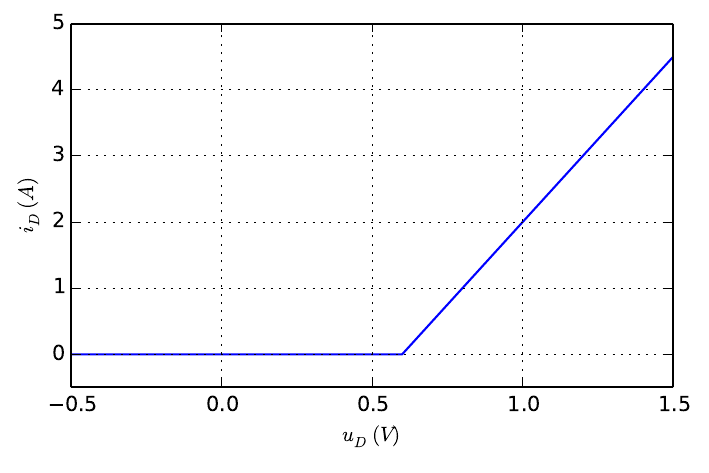
\includegraphics[width=\linewidth]{diode_annexe}
		\caption{}
		\label{fig:annexe_e2}
	\end{figure}

	\chapter*{Annexe~: problème 2}

	\begin{figure}[htbp!]
		\centering
		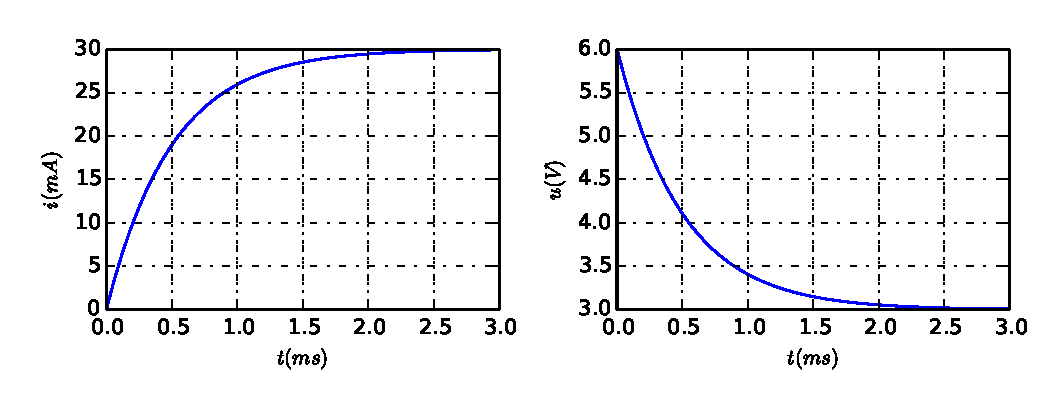
\includegraphics[width=\linewidth]{transRL_trace.pdf}
		\caption{Annexe question 6.}
		\label{fig:annexe_p2-1}
	\end{figure}
	\begin{figure}[htbp!]
		\centering
		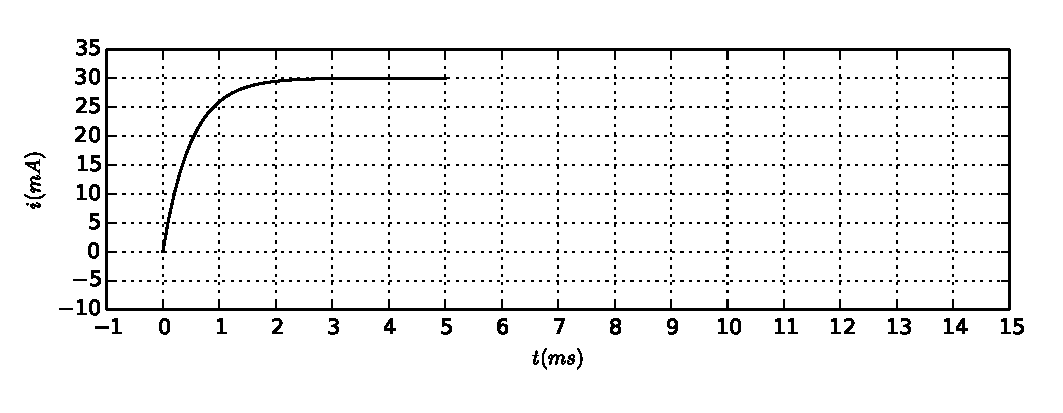
\includegraphics[width=\linewidth]{transRL_tracei.pdf}
		\caption{Annexe question 17.}
		\label{fig:annexe_p2-2}
	\end{figure}
	\begin{figure}[htbp!]
		\centering
		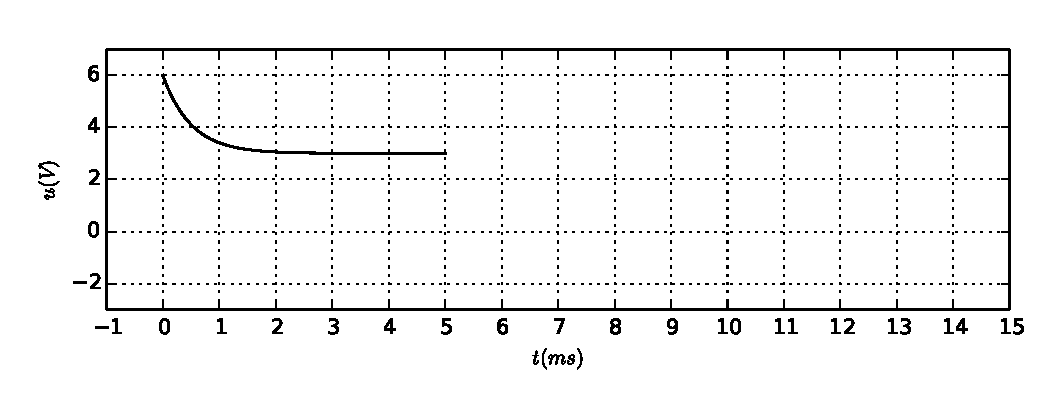
\includegraphics[width=\linewidth]{transRL_traceu.pdf}
		\caption{Annexe question 18.}
		\label{fig:annexe_p2-3}
	\end{figure}

}{
	\newpage
	\chapter*{Annexe~: exercice 2}


	\chapter{Annexe~: problème 2}
	\begin{center}
		\subimport{figures/P2/}{transRL_tracecorr.pdf}
		\captionof{figure}{Annexe question 6.}
		\label{fig:annexe_p2-1_corr}
	\end{center}
	\begin{center}
		\subimport{figures/P2/}{transRL_traceicorr.pdf}
		\captionof{figure}{Annexe question 6.}
		\label{fig:annexe_p2-2_corr}
	\end{center}
	\begin{center}
		\subimport{figures/P2/}{transRL_traceucorr.pdf}
		\captionof{figure}{Annexe question 6.}
		\label{fig:annexe_p2-3_corr}
	\end{center}
}
\vspace{-20pt}
\end{document}
